\documentclass[12pt]{article}

% House style preamble: central symlink only.
\input{.house-style/preamble.tex}

% Anonymization toggle for double-blind review.
\newif\ifblind
\ifdefined\blindbuild \blindtrue \else \blindfalse \fi

\hypersetup{
  pdftitle={Was magnitude estimation necessary? A secondary-data reassessment of Bard, Robertson, and Sorace (1996)},
  pdfkeywords={magnitude estimation, acceptability judgments, grammaticality judgments, secondary data, experimental syntax}
}
\ifblind\hypersetup{pdfauthor={}}\fi

\title{Was magnitude estimation necessary?\\
{\large A secondary-data reassessment of Bard, Robertson, and Sorace (1996)}}
\ifblind
  \author{[Author name, ORCID, and affiliation removed for double-blind review]}
\else
  \author{Brett Reynolds \orcidlink{0000-0003-0073-7195}%
  \thanks{Contact: \href{mailto:brett.reynolds@humber.ca}{brett.reynolds@humber.ca}}\\
  Humber Polytechnic \& University of Toronto}
\fi
\date{June 2026}

\begin{document}
\maketitle

\begin{abstract}
This paper reassesses Bard, Robertson, and Sorace's case for magnitude
estimation in linguistic acceptability research. It separates two claims that
are often run together: acceptability judgments are graded, measurable, and
methodologically serious; magnitude estimation has a practical advantage over
simpler formal judgment tasks. The first claim is the stronger legacy. The
second requires later method-comparison evidence.

The paper reports a constrained, prespecified secondary analysis of Sprouse and
colleagues' public method-comparison data, now within an approved data-reuse
boundary. The reanalysis finds strong cross-method convergence and bounded
response-function curvature, but no systematic practical resolution advantage
unique to magnitude estimation. Langsford et al.\ enter as article-level
evidence about reliability and response-style risks, while computational
benchmarks remain afterlife evidence rather than evidence about magnitude
estimation itself.
\end{abstract}

\noindent\textbf{Keywords:} magnitude estimation; acceptability judgments; grammaticality judgments; secondary data; experimental syntax

\section{The problem}

Bard, Robertson, and Sorace made a methodological claim that was larger than a
single elicitation format. Acceptability judgments, they argued, could be
treated as graded measurements rather than as informal binary verdicts
\citep{BardEtAl1996}. That move helped make experimental syntax a
measurement enterprise: judgments could be collected from naive participants,
scaled, compared across groups, and subjected to ordinary statistical tests.

Whether magnitude estimation was necessary for that advance is a harder
question.
Magnitude estimation promised a way around the scale restrictions of
traditional judgment tasks, giving participants an open response scale and
preserving fine distinctions. But later acceptability work didn't settle into
one privileged elicitation method. Likert ratings, forced choice, yes/no tasks,
and Thurstonian models all became part of the measurement toolkit
\citep{sprouse2013,LangsfordEtAl2018,sprouse2017}.

This paper separates two claims that are often allowed to travel together. One
claim is strong and still plausible: acceptability is graded, measurable, and
methodologically serious. The other is weaker: magnitude estimation has a
practical measurement advantage over simpler formal tasks. The first claim can
survive even if the second doesn't.

This empirical question isn't new. The methodology literature has already
compared elicitation formats and largely deflated magnitude
estimation's special status. \textcite{schutze2016} reports that most or all of
its advertised advantages over Likert tasks have since been refuted, pointing to
\textcite{weskott2011} and \textcite{sprouse2013}; later work weighed the formats
on convergence \citep{sprouse2013}, statistical power \citep{sprouse2017},
and reliability and response style \citep{LangsfordEtAl2018}.

This paper instead contributes a clearer routing of the evidence. Existing
method-comparison work already weakens magnitude estimation's special status;
the reassessment asks what the
surviving formal-judgment signal licenses us to project. In the approved
reanalysis of the 2013 and 2017 comparison data and a post-outcome robustness
multiverse, formal judgment
formats preserve stable item-level contrast ordering across the tested
contrasts, while magnitude estimation adds no robust separate practical
ordering there.

Seen this way, the reassessment doesn't reject Bard et al.'s programme. It
tests what should be credited to magnitude estimation itself, and what
should instead be credited to the broader formalization of acceptability
judgment methodology.

\section{The Bard target}

Reassessing Bard et al.\ means first stating, from the article rather than its
reputation, what they actually claimed. The abstract makes four claims for
magnitude estimation: that it can \enquote{solve the measurement scale problems
which plague conventional techniques}, \enquote{provide data which make fine
distinctions robustly enough to yield statistically significant results of
linguistic interest}, be \enquote{usable in a consistent way by linguistically
naive speaker-hearers}, and \enquote{allow replication across groups of
subjects} \citep[32]{BardEtAl1996}.

The core of the case is an argument about scale type, not about reliability.
The trouble with conventional annotation, they argue, is \enquote{the use of the
wrong kind of measurement scale} \citep[32]{BardEtAl1996}: the asterisk
system, like any fixed-point scale, \enquote{predetermines the number of
distinctions subjects may use} and so censors finer ones
\citep[35]{BardEtAl1996}. Magnitude estimation is the proposed remedy
because it \enquote{does not restrict the number of values}, giving subjects
\enquote{complete freedom about which of the infinite set of numbers to use} and
yielding interval and ratio data \citep[41]{BardEtAl1996}.

This sharpens Bard et al.'s claim and its boundary. They do make a
method-superiority claim, but a specific one: an open, ratio-yielding response
recovers gradient distinctions that fixed-point scales lose by construction.
The claim concerns resolution and scale-boundary censoring, and it can be
tested. The broader reading sometimes met in reception, that magnitude
estimation is the privileged formal method in general, goes beyond the article;
Bard et al.\ compare magnitude estimation with informal annotation and
fixed-point scales, not with the later inventory of Likert, forced-choice,
yes/no, and Thurstonian tasks.

Bard et al.\ are also more tentative than the reception. They grant that the
advantages \enquote{are garnered at considerable empirical cost}, and they leave
open which psychological model underlies acceptability, since \enquote{the data
currently do not decide between them} \citep[65]{BardEtAl1996}. The fair
target for reassessment is the resolution claim, not a gold-standard claim the
authors didn't make.

The distinction matters for design. If the live claim is that an open ratio
scale recovers distinctions fixed scales censor, then the later method
comparisons have to test resolution and scale-boundary effects alongside
convergence and reliability. Because Bard participant-level rows aren't
available to this project, the paper can't replicate the original experiment
directly; the reassessment is a conceptual replication and secondary-data test
of whether the resolution claim retains independent evidential force.

\section{Secondary-data design}

The secondary-data design treats the project as a measurement reassessment of
Bard, Robertson, and Sorace \citep{BardEtAl1996}. It separates four kinds of
source from the observation channels introduced in
Section~\ref{sec:gramm-accept}: sources are routed to estimands, while channels
bear on grammatical inferences. Published summaries from Bard et al.\ can source
the historical claim, but can't support a direct replication without their
participant-level data.

Later judgment studies can support secondary analysis when they compare
elicitation methods on shared or comparable items and provide the rows needed
for the intended estimand. Computational benchmarks can show the afterlife of
acceptability labels, but they don't bear on magnitude estimation versus
Likert ratings. Construct-level discussion can separate acceptability from
grammaticality, naturalness, standardness, and correction.

\begin{table}[H]
\centering
\small
\begin{tabular}{@{}>{\raggedright\arraybackslash}p{0.19\linewidth}>{\raggedright\arraybackslash}p{0.22\linewidth}>{\raggedright\arraybackslash}p{0.25\linewidth}>{\raggedright\arraybackslash}p{0.24\linewidth}@{}}
\toprule
Source & Evidence level & Use in this paper & Unsupported claim \\
\midrule
Bard et al.\ 1996 & Published article & Historical target and scale-resolution claim & Direct replication without participant rows \\
Sprouse, Sch\"utze, and Almeida 2013; Sprouse and Almeida 2017 & Public row-level comparison data & Constrained secondary method comparison within approved reuse boundary & Raw-data redistribution or drift beyond the approved methodological scope \\
Langsford et al.\ 2018 & Published article and supplement & Reliability and response-style synthesis & New participant-level reliability model without raw rows \\
CoLA, BLiMP, SAD & Benchmark labels and documentation & Afterlife of formal acceptability measurement & Evidence about ME versus other human judgment methods \\
\bottomrule
\end{tabular}
\caption{Evidential routing before analysis. ME = magnitude estimation; SAD =
Syntactic Acceptability Dataset.}
\label{tab:evidence-routing}
\end{table}

The approved reuse boundary resolves the secondary-data side of the genre gate.
Public row-level data from the two comparison studies support a constrained
secondary analysis of method performance. The original studies had different
aims: \textcite{sprouse2013} estimated convergence between informal and formal
judgments, while \textcite{sprouse2017} studied task sensitivity and statistical
power. The present resolution analysis is a secondary use of their rows, not a
claim about what those studies were designed to test.

The verified public Langsford materials available to this project lack raw
participant responses. This limits Langsford et al.\ to the article-summary
level; the analysis doesn't attempt a participant-level
response-style or test-retest model across the literature.

The comparison files also require representation choices before modelling. For
the 2013 data, the primary forced-choice comparison uses the pair-level sign-test
file because forced choice is a pairwise task and that file records judgments
against expected patterns. The logistic file preserves item-level binary rows
and changes the unit of analysis, so it serves as a named sensitivity
specification.

For the 2017 data, yes/no rows with item IDs \texttt{B}, \texttt{G}, and
\texttt{M} are excluded from item-level comparisons.
They're absent from the materials workbook, occur in repeated early order
positions for every subject, and don't align with the magnitude-estimation,
Likert, or forced-choice item universe. This exclusion is a structural
inclusion rule, not an outcome-based trimming decision.

Each source is assigned to an estimand it can answer. The primary estimand is
the item-level acceptability signal
recoverable across methods. Secondary estimands are method-specific noise or
bias and decision agreement for theoretically relevant contrasts.

Participant response style and method-by-item instability are admissible only
when the dataset contains the participant-level rows and repeated structure
needed to estimate them. This ordering keeps the analysis from selecting
whichever scale looks best after the fact, the kind of forking path Gelman and
Loken warn about \citep{GelmanLoken2013,gelman2014statcrisis}.

The substantive comparison uses a measurement null, but a careful one. Magnitude
estimation, Likert ratings, forced choice, and Thurstonian choice are modelled
as readings of a common item-level acceptability signal through method-specific
response functions, not as the same signal plus method noise: the bounded
methods can compress the signal at the extremes, while the open ratio scale need
not. The single-dimension assumption is checked before any
method-specific term is read. With richer row-level evidence, that check would
compare a one-factor model against correlated-two-factor and bifactor
alternatives and inspect method residuals for item-level structure. In the
present reanalysis, the implemented counterpart is deliberately weaker:
a first-pass PCA/parallel-analysis check over aggregate item and contrast
matrices.

This ordering matters because the advantage Bard et al.\ actually claimed is
about resolution, recovering distinctions that fixed scales censor
\citep[35]{BardEtAl1996}. A plain common-signal-plus-noise null would book
that resolution as magnitude-estimation noise and let the method only lose; the
response functions and the dimensionality check let a resolution advantage
register instead. If one factor suffices, magnitude estimation still has to earn
its term; if it doesn't, the analysis turns to where the methods diverge.
Scrambled labels, method-label permutations, and simulations from the
response-function model would be pipeline controls rather than substantive
comparisons; the paper doesn't use them as evidence about ME.

After the chartered analyses were complete, a bounded multiverse tested whether
their conclusion depended on defensible representation choices. Its
specification universe was frozen before that analysis was run, but after the
primary outcomes were known, so it's a post-outcome robustness analysis rather
than a prespecified test. Three families vary ME and Likert scoring, endpoint
definitions and spread measures, raw- and rank-scale prediction, and independent
forced-choice or yes/no adjudication. The resulting 162 specifications test
scale-boundary spread, incremental out-of-sample information, and actual
contrast-sign disagreements without treating unexplained ME variance as an
advantage by itself. The complete decision rules and specification list are
versioned in \texttt{notes/sprouse-resolution-multiverse-plan.md}.

\section{Scale and reliability}

The scale question is practical measurement advantage over
the response-function measurement null set out in the secondary-data design.
Bard et al.'s case for magnitude estimation included scale resolution,
fine-grained distinctions, naive-participant use, and replication across groups
\citep[32]{BardEtAl1996}. The safer target is that source-grounded claim,
together with the stronger reading of magnitude estimation that took hold in
parts of the later methodology literature.

Later method-comparison data give the paper a sharper question: does magnitude
estimation recover item differences, participant agreement, or theoretically
relevant decisions that simpler tasks lose, and in particular does it recover
graded distinctions that bounded scales compress at the extremes?

\textcite{sprouse2013} compare formal judgment tasks with informal published
judgments, giving evidence about convergence between magnitude estimation,
Likert ratings, and forced choice. The public rows from that study can support a
bounded reanalysis of item-level agreement and decision consequences within
the approved reuse boundary. \textcite{LangsfordEtAl2018} add a reliability and
response-bias target by comparing Likert, magnitude estimation, forced choice,
and Thurstonian models. Without their raw rows, Langsford can support the
synthesis of published reliability findings but not a new participant-level
response-style or test-retest model.

The reanalysis inherits the unit-of-analysis charter fixed in the secondary-data
design rather than reopening it. The same primary and sensitivity
representations carry over, so the claims stay traceable to fixed units of
analysis instead of to whichever representation later proves most convenient.

The primary comparison weighs methods on resolution, prediction, decision
consequences, and convergence, prioritizing consequences for the linguistic
contrast. Resolution is the criterion Bard's claim lives on: whether magnitude
estimation recovers graded item differences that bounded scales compress at
ceiling or floor, or a measurement dimension that survives the dimensionality
check. Reliability is a distinct property, not a proxy for it;
\textcite{LangsfordEtAl2018} report magnitude estimation as less reliable, which
doesn't by itself settle resolution.

For this paper, a practical magnitude-estimation advantage would have to change
an inferential decision. A summary-statistic improvement alone wouldn't count.
An advantage would count if magnitude estimation recovered a good-vs-bad contrast that
bounded methods missed, showed its largest extra spread exactly where bounded
scales compressed the response, carried a stable method-specific dimension
across scoring choices, or reduced sign-error or exaggeration risk for a named
contrast under a design analysis. A larger correlation, by itself, wouldn't
settle the question.

The reanalysis of both comparison datasets gives a narrow answer. Magnitude
estimation and the bounded methods share a strong aggregate item-level signal. Raw Likert means
also show the expected bounded response-function curvature relative to magnitude
estimation. That curvature is the pattern Bard's scale argument makes visible,
but the endpoint and pair-level diagnostics don't show a systematic practical
distinction preserved only by magnitude estimation.

Figure~\ref{fig:response-functions} makes the common signal and bounded
curvature visible. The linear fit tracks the centre of each cloud but runs past
the Likert scale's upper boundary, while the bounded fit turns towards that
boundary. That pattern is why the analysis allows method-specific response functions
before asking whether magnitude estimation preserves a further practical
distinction.

\begin{figure}[H]
\centering
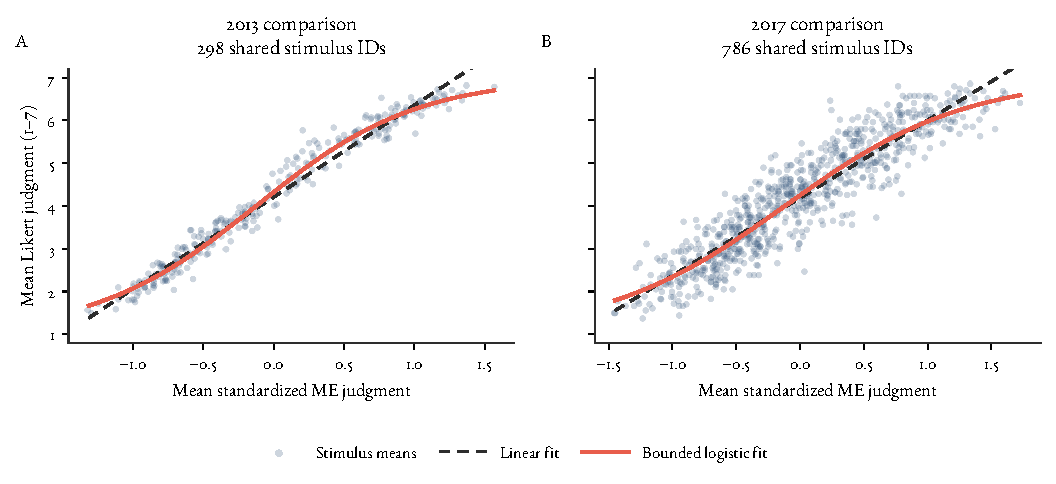
\includegraphics[width=\linewidth]{figures/response-functions.pdf}
\caption{Aggregate response functions in the public comparison data from
Sprouse, Sch\"utze, and Almeida (2013) (A) and Sprouse and Almeida (2017) (B).
Each point averages participant judgments for one stimulus identifier shared by
the magnitude-estimation and Likert files. The 2013 files call these identifiers
\enquote{conditions} (298 points); the 2017 files call them \enquote{items} (786
points). The two labels reproduce the source-file nomenclature. The dashed line
is a linear fit and the solid line is a 1--7 bounded logistic fit. Magnitude
estimation is an unbounded diagnostic axis here, not the assumed true latent
acceptability scale.}
\label{fig:response-functions}
\end{figure}

The dimensionality result is deliberately modest: a first-pass aggregate
check of the item and contrast matrices, used to ask whether a clear
multidimensional rescue for magnitude estimation appears in the available
aggregate summaries. It doesn't replace a full participant-level factor model,
which would require a broader row-level evidence base than this paper has.

The rows in Table~\ref{tab:sprouse-diagnostics} come from the approved pipeline
documented in \texttt{analysis/README.md}: item-signal, dimensionality,
response-function, pair-robustness, and aggregate sensitivity scripts. The
reported \(n\) values are aggregate condition, item, or pair units, not
participant-level rows. A 95\% percentile bootstrap over those same aggregate
units gives intervals that leave the interpretation unchanged: ME--Likert
correlations remain high for 2013 conditions [.983, .989], 2013 pairs [.950,
.974], 2017 items [.915, .934], and 2017 pairs [.917, .965], and pair-level
bounded-predictor \Rsq{} remains high for 2013 [.900, .946] and 2017
[.862, .941].

\begin{table}[H]
\centering
\small
\renewcommand{\arraystretch}{1.08}
\begin{tabular}{@{}>{\raggedright\arraybackslash}p{0.23\linewidth}>{\raggedright\arraybackslash}p{0.34\linewidth}>{\raggedright\arraybackslash}p{0.34\linewidth}@{}}
\toprule
Diagnostic & 2013 study & 2017 study \\
\midrule
ME--Likert convergence & Conditions \(n=298\), \(r=.986\); pairs \(n=150\), \(r=.963\) & Items \(n=786\), \(r=.925\); pairs \(n=50\), \(r=.944\) \\ \addlinespace[2pt]
First-pass dimensionality check & Pairs \(n=150\): first component 89.4\%; second eigenvalue below parallel-analysis threshold & Items \(n=786\), pairs \(n=50\): first components 80.6\% and 85.9\%; second eigenvalues below thresholds \\ \addlinespace[2pt]
Bounded response function & Conditions \(n=298\): bounded logistic improves over linear; endpoint ME SDs .142 and .175 versus middle .313 & Items \(n=786\): bounded logistic improves over linear; endpoint ME SDs .249 and .321 versus middle .349 \\ \addlinespace[2pt]
Pair robustness & Pairs \(n=150\): bounded predictors \Rsq{} = .926; no ME top-quartile pair falls in the bounded bottom half & Pairs \(n=50\): bounded predictors \Rsq{} = .901; no ME top-quartile pair falls in the bounded bottom half \\
\bottomrule
\end{tabular}
\caption{Primary diagnostics from the comparison data accompanying Sprouse,
Sch\"utze, and Almeida (2013) and Sprouse and Almeida (2017) for Bard's
resolution claim. ME = magnitude estimation. The dimensionality row is an
aggregate first-pass check,
and the response-function rows use magnitude estimation as an unbounded
diagnostic axis rather than the true latent acceptability scale.}
\label{tab:sprouse-diagnostics}
\end{table}

Table~\ref{tab:sprouse-diagnostics} separates three facts. First, the
aggregate matrices provide no obvious multidimensional rescue for magnitude
estimation. Second, the Likert scale behaves like a bounded response function,
so a fair null should allow compression. Third, the available contrasts
don't show the further pattern that would make magnitude estimation
practically superior: endpoint regions aren't where magnitude estimation
spreads out most, and good-vs-bad pairs ranked highly by magnitude estimation
are also ranked highly by bounded methods.

The explicitly post-outcome multiverse asks whether that interpretation survives
defensible scoring and modelling choices. It varies three ME scores, three
Likert scores, endpoint definitions and spread statistics, raw- and rank-scale
prediction, and forced-choice or yes/no adjudication. None of its endpoint,
incremental-prediction, or decision-adjudication families meets the frozen
family-level criterion in either dataset.

The disaggregated result contains one useful qualification. Both endpoint ratios
exceed one in 3 of 27 specifications for 2013 and 6 of 27 for 2017; only one 2017
specification also clears the practical and permutation criteria. ME adds at
least .02 cross-validated \Rsq{} beyond Likert in 0 of 36 prediction
specifications for 2013 and 4 of 36 for 2017. Those four are rank-scale models
of forced choice (\deltaRsq{} = .025--.049); the increment doesn't generalize
to 2017 yes/no judgments or to raw-scale mappings. ME and Likert disagree on
the contrast sign for only 3 of 150 pairs in 2013 and 1 of 50 in 2017, too few
to clear the decision criterion. The localized 2017 result makes a blanket
no-information claim too strong for those specifications, but it doesn't
establish a systematic practical advantage.

Figure~\ref{fig:multiverse-landscape} shows why the qualification matters
without changing the family-level conclusion. The isolated endpoint result and
four prediction increments sit inside distributions dominated by smaller or
negative effects, while actual ME--Likert contrast-sign disagreements remain
rare.

\begin{figure}[H]
\centering
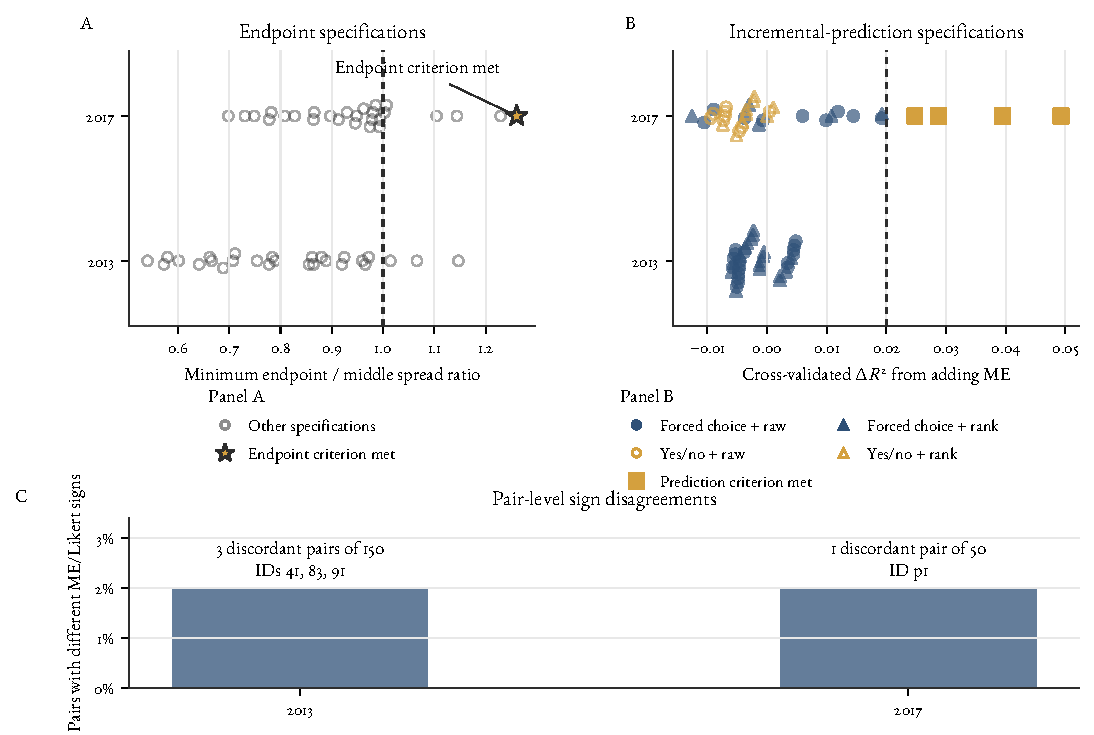
\includegraphics[width=\linewidth]{figures/multiverse-landscape.pdf}
\caption{The explicitly post-outcome multiverse. Panel A shows all 54 admissible
endpoint specifications; the dashed line marks equal minimum endpoint and
middle spread. The golden star is the sole specification in which both endpoint
ratios reach 1.25 and the permutation probability is below .05. Panel B shows
all 72 incremental-prediction specifications. Filled blue markers denote a
forced-choice target and open golden markers a yes/no target; circles denote
raw-scale mappings and triangles rank-scale mappings. Solid golden squares mark
the four specifications meeting the prediction criterion: \deltaRsq{} from
adding ME is at least .02 and exceeds the corresponding increment from adding
Likert. The dashed line marks the .02 threshold. Symmetric vertical stacking
separates nearby specifications; vertical position within a study row has no
substantive meaning. Panel C shows the proportion of pairs on which ME and
Likert disagree about the contrast sign; it uses pair rows rather than the
specification counts in Panels A and B. The disagreements are invariant across
all nine ME--Likert scoring combinations: 2013 pair IDs 41, 83, and 91 account
for 3 of 150 pairs, and 2017 pair ID p1 accounts for 1 of 50. No decision
specification clears its family rule.}
\label{fig:multiverse-landscape}
\end{figure}

These aggregate practical diagnostics are weaker than posterior certainty
statements or formal equivalence tests. They show that the available contrasts
lack the predicted ME-only pattern; they leave open participant-level method
factors, response-style dimensions, and locally dependent item effects.

Type S and Type M errors enter only as properties of estimating a named contrast
at a given sample size, not as properties a format carries. The relevant
question is whether choosing magnitude estimation rather than another method
changes the sign-error probability or the exaggeration ratio for a specific
contrast under a design analysis \citep{gelman2014types}. Sensitivity checks
are reported as named specifications rather than invisible post hoc
choices \citep{steegen2016increasing}. The multiverse follows that rule, but
its timing still makes it a robustness analysis rather than a preregistration.

\section{The contemporary afterlife of acceptability}

TODO: Treat modern benchmark resources as an afterlife of acceptability, not as
direct magnitude-estimation evidence. Resources such as BLiMP
\parencite{WarstadtEtAl2020} and the Syntactic Acceptability Dataset
\parencite{juzek2024} show how acceptability became portable for computational
evaluation, but they also change the object being measured.

\section{Grammaticality and acceptability}\label{sec:gramm-accept}

The reassessment also needs a disciplined vocabulary. The background view
adopted here is that grammar is a system of projectibility profiles
\citep{Goodman1955}: relatively stable patterns that license explicitly
scoped inferences from forms, meanings, contexts, speakers, and judgments to
uses a community or register treats as available. Research purposes select
which inference is worth testing; they don't make the inference true.

The empirical projective claim in this paper is deliberately narrow. For the
sampled contrasts in the 2013 and 2017 comparison data, observing relative
ordering under one formal elicitation format warrants expecting similar
aggregate ordering under another,
within the variation reported here. A grammaticality claim has wider targets:
interpretation, production, correction, expert classification, register fit,
cross-speaker stability, and related consequences. Those targets require data
beyond the task-format comparisons analysed in this paper.

The paper distinguishes three observation channels from the target. Participant
responses under an acceptability prompt are observations of judgments under a task. Expert
asterisks and published example labels are classifications made within a
theoretical or editorial practice. Benchmark labels are dataset-construction
decisions. The projectibility profile is the target: the structure of inferences
a form licenses, what its acceptability, production, correction, expert
classification, register fit, and cross-speaker stability jointly project to. Two
channels are evidence about the same profile when they bear on the same form's
inferential relations.

So the profile isn't the average of the channels, and channel disagreement is
not noise to smooth away. When a sentence is rated low by naive participants,
left unstarred in the literature, and attested in a register corpus, the verdict
about its profile is fixed by which inferences actually hold, tested against
further data, not by a vote across channels.

A channel that consistently fails to predict the others establishes divergence,
not its interpretation. Independent evidence has to decide whether the divergence
reflects task specificity, noise, or a distinct part of the profile. That
requirement makes the profile more than an unweighted set of labels and supplies the identity
condition the level discipline needs.

This discipline keeps neighbouring constructs apart. Acceptability is one
evidential route into a projectibility profile, not the profile itself. Personal
production, naturalness, standardness, correction behaviour, and theoretical
classification project differently. A sentence can be dispreferred without
being ungrammatical, correctable without being unnatural, or standard in one
register while unacceptable under another task framing.

The framing earns its place in the measurement argument by predicting where a
single task-conditioned acceptability scalar could be insufficient: items where
participants rate a sentence low but the literature leaves it unstarred, or
where the form is standard in one register and degraded under another task
framing. A dataset that samples those channels jointly should put a
single-scalar model at risk.

The present comparison matrices contain formal task responses rather than that
cross-channel evidence. They test the narrower question of whether ME
carries a stable method-specific dimension or practical ordering that the
bounded tasks miss. The projectibility account supplies a wider empirical
programme, but the paper doesn't treat the task-format result as having already
tested it.

Bard et al.\ helped make one part of this space measurable: graded
acceptability judgments from participants \citep{BardEtAl1996}. Their work made a
major contribution to the measurement of one evidential channel. It doesn't by
itself show that an acceptability scale captures every inference licensed by a
grammar. Later benchmarks sometimes repackage acceptability-related labels as
grammaticality targets \citep{WarstadtEtAl2019CoLA,WarstadtEtAl2020}. The
Syntactic Acceptability Dataset is valuable here because it explicitly
separates literature-derived grammatical status from crowd acceptability status
\citep{juzek2024}.

That boundary also limits the no-new-data paper. Existing datasets can compare
the stability of elicitation methods and clarify how acceptability labels
travel. They can't settle a full projectibility profile for a construction:
production, correction, register, interpretation, and community licensing would
require data designed for those inferences.

\section{Conclusion}

A balanced update is straightforward. Bard et al.\ were right to insist that
acceptability could be treated as measurable and methodologically serious. Their documented case
for magnitude estimation concerned scale resolution, fine distinctions,
naive-participant use, and replication across groups
\citep[32]{BardEtAl1996}. That claim deserves credit as part of the
history of experimental syntax.

Method-specific conclusions require more restraint and a fair test.
Magnitude estimation is compared against a measurement null in which later
formal tasks read a common item-level acceptability signal for the analysed
contrasts through method-specific response functions, and in which the
single-dimension assumption is checked before any method-specific term is
read. The question is then whether magnitude estimation earns its keep on
resolution, the distinctions Bard argued fixed scales censor, or on prediction,
decision stability, or construct interpretation, rather than whether it survives
a null that books resolution as noise.

The approximation uses aggregate matrices from the two comparison studies,
response-function diagnostics, pair-level robustness checks, and a bounded post-outcome
multiverse. Its scope matters because the participant rows needed for a full
dimensionality model across Bard, Sprouse, and Langsford aren't available to
this project.

The reanalysis supports that update. Across the two comparison datasets,
magnitude estimation and the bounded methods share a strong aggregate practical
signal. First-pass aggregate
dimensionality checks show no obvious evidence against a single dominant
dimension at that level of aggregation. Raw Likert means show bounded
response-function curvature, which is exactly why the null shouldn't treat
bounded tasks as simple noisy copies of magnitude estimation.

By contrast, the remaining resolution diagnostics are less favourable to the
stronger method claim: endpoint regions don't show unusually large magnitude-estimation
spread, and pair-level bounded predictors recover most magnitude-estimation
contrast variance. None of the three multiverse families clears its frozen
cross-specification criterion in either dataset. Four 2017 rank-scale
forced-choice specifications show a small ME increment, but that result doesn't
generalize to yes/no judgments, raw-scale mappings, or the 2013 data. Langsford
et al.\ remain article-level evidence because their raw responses aren't
available to this project.

Projectibility adds a correspondingly modest payoff. Within the sampled
contrasts in the two comparison datasets, observing relative ordering under one
formal task warrants expecting similar aggregate ordering under another.
Magnitude estimation alone doesn't
support an additional robust practical ordering for those contrasts. The result
warrants a task-format inference, not the claim that every grammatical inference travels
across speakers, registers, or observation channels.

The conclusion would change under a clear ME-only pattern: endpoint regions
with much larger ME spread than middle regions, high-ME contrasts that bounded
methods consistently placed low, stable method-specific residual structure
across scoring choices, or lower sign-error and exaggeration risk for named
linguistic contrasts. Those are the patterns the present diagnostics do
not show.

Across these checks, the central conclusion remains stable. The durable legacy is the formal
measurement of graded acceptability as one route into grammar's projectibility
profiles. The broader privileged status sometimes read into magnitude
estimation is a separate claim, and later evidence has to earn it separately.


\section*{Data and code availability}

No raw participant-level data is committed to this repository. Source and
dataset verification are tracked in \texttt{notes/source-verification.md}; the
analysis charter and structural Sprouse inventory are tracked in
\texttt{notes/analysis-charter.md} and \texttt{notes/dataset-inventory.md}.
Sprouse reuse permission has been approved for the limited secondary
methodological analysis described in the charter. Scripts generate ignored local
structural derivatives, readiness manifests, and descriptive item/contrast
signal, dimensionality, response-function, and pair-level robustness outputs
under \texttt{data/derived/}; participant-level raw files remain outside the
repository.

\section*{Acknowledgements}

TODO: Add final AI-use disclosure with the actual model list used on the
project.

\clearpage
\printbibliography

\end{document}
